\begin{figure}[t!]
  \centering
    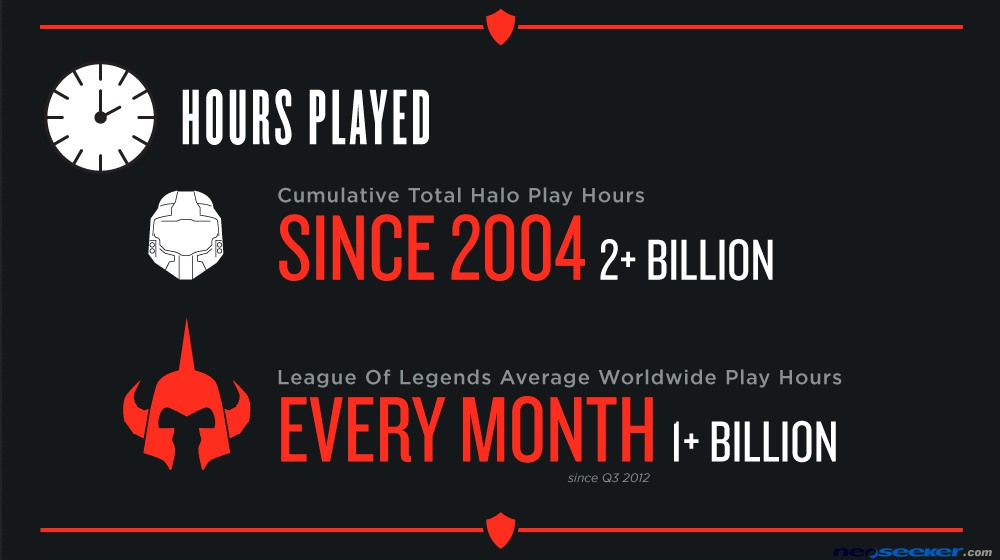
\includegraphics[width=0.5\textwidth]{increased-gaming}
  \caption{League of Legends has soared in popularity recently, accumulating more play time per month than a rival game has since its release.  These numbers are continually increasing \cite{1_riot_games_2015}.}
  \label{fig:increased-gaming}
\end{figure}

\section{Introduction}
Machine Learning and Big Data have been hot, related topics in Computer Science.
Machine learning models benefit greatly from large amounts of data 
available for training and testing, and their applications are being used in varying fields 
of research and industry.  One of the most common use cases is to train a classifier, which 
can classify an input as a certain category.

Machine learning has been prevalent in the traditional sports setting for many different use 
cases ranging from something as general as predicting the winner of a game, to predicting something 
specific such as the score of a game, and to even predicting all the outcomes of the games in a 
tournament bracket.  Examples of the latter include the sophisticated models by Bloomberg to predict 
the World Cup with 16 teams and 32 games in a single-elimination tournament \cite{4_bloomberg_2015}.  

With the rise of popularity of electronic sports (eSports) and competitive gaming, 
there is potential to draw a parallel in applications between eSports and traditional sports.  
In particular, League of Legends, an online multiplayer game, is one of the top contenders for 
the most professional and developed competitive eSport.  Professional teams for League of Legends 
operate similar to traditional sports teams, and they have begun hiring coaches and analysts to 
help them improve their gameplay.
These games generate tons of data that can be analyzed in a way 
similar to the results of sports games, potentially giving an advantage to the teams 
with better data analysis. 

Our work applies some 
machine learning techniques on the data available for League of Legends, and we show that
we can extract useful insights to predict win-rates.

\textbf{ Contributions.} Our contributions are summarized as follows:
\begin{itemize}
\item We apply machine learning techniques such as Sparse Coding, Support Vector Machines (SVM), 
and Random Forests on accumulated League of Legends 
game data to accurately predict win-rates for games. 
\item We introduce the idea of using a player's match history as an input to machine learning 
models as a training feature.
\item We demonstrate a framework to collect and aggregate data to feed into our machine learning model.
\end{itemize} 
